% ============================================================================
% Defence Guide: speaking about the project with confidence
% Research project: "Learning What to Remember for Time-Series Prediction
% Using Reinforcement Learning"
%
% Compile (from Windows):  ..\build.bat defence\defence_guide.tex
% Output lands in defence\build\defence_guide.pdf
% Figures it needs: ../plots/..., ../results/rq1_lstm_sweep/seed_7/...,
%                   ./figures/... (made by make_defence_figures.py)
% ============================================================================
\documentclass[11pt,a4paper]{article}
\usepackage[margin=2.3cm]{geometry}
\usepackage[T1]{fontenc}
\usepackage{lmodern}
\usepackage{amsmath,amssymb}
\usepackage{graphicx}
\usepackage{booktabs}
\usepackage{longtable}
\usepackage{array}
\usepackage{enumitem}
\usepackage{xcolor}
\usepackage[most]{tcolorbox}
\usepackage{tikz}
\usepackage{hyperref}
\usepackage{titlesec}

\graphicspath{{../plots/}{../results/}{./figures/}}
\setlist{itemsep=2pt,topsep=4pt}
\setlength{\parskip}{5pt}
\setlength{\parindent}{0pt}
\hypersetup{colorlinks=true,linkcolor=blue!50!black,urlcolor=blue!50!black}
\titleformat{\section}{\normalfont\Large\bfseries}{\thesection}{0.8em}{}
\titleformat{\subsection}{\normalfont\large\bfseries}{\thesubsection}{0.6em}{}

% ---------- boxes ----------
% "Say it" : words you can say out loud in the meeting.
\newtcolorbox{sayit}{colback=green!4,colframe=green!45!black,boxrule=0.6pt,
  left=6pt,right=6pt,top=4pt,bottom=4pt,title={\small\bfseries Say it like this},fonttitle=\small}
% "Be honest" : a weakness you raise yourself before he finds it.
\newtcolorbox{honest}{colback=orange!5,colframe=orange!70!black,boxrule=0.6pt,
  left=6pt,right=6pt,top=4pt,bottom=4pt,title={\small\bfseries Be honest about this},fonttitle=\small}
% "Axes" : how to read a figure, in order.
\newtcolorbox{axes}{colback=blue!3,colframe=blue!45!black,boxrule=0.6pt,
  left=6pt,right=6pt,top=4pt,bottom=4pt,title={\small\bfseries How to read it},fonttitle=\small}
% "Q" : a question he may ask, and an answer.
\newtcolorbox{qa}[1]{colback=gray!4,colframe=gray!55!black,boxrule=0.5pt,
  left=6pt,right=6pt,top=4pt,bottom=4pt,title={\small\bfseries Q: #1},fonttitle=\small}

\newcommand{\fig}[2]{\begin{center}\includegraphics[width=#2\linewidth]{#1}\end{center}}

\title{\vspace{-1.5cm}\textbf{Defence Guide}\\[4pt]
\large Learning What to Remember for Time-Series Prediction Using Reinforcement Learning\\[2pt]
\normalsize Everything you need to explain the project, the plots, and the numbers, in plain words}
\author{Banele Mkhize \quad (supervisor: Geraud Nangue Tasse)}
\date{October 2026}

\begin{document}
\maketitle
\vspace{-0.6cm}

\tableofcontents
\newpage

% ============================================================================
\section*{How to use this guide}
\addcontentsline{toc}{section}{How to use this guide}

You froze last time because three things were missing at once: the meaning of the
short labels (h64L1, hp2, k=3), the meaning of the axes, and a sentence ready to say
about each plot. This guide fixes all three.

Read it in this order:
\begin{enumerate}
  \item Section 1 (the 30-second version). Learn it until you can say it without looking.
  \item Section 3 (every label and abbreviation). This is the part that froze you.
  \item Section 6 (the 868 models, seeds, windows). This is what Geraud asked about.
  \item Section 8 (plot by plot). One page per plot. Each has a ``how to read it'' box
        and a ``say it like this'' box.
  \item Section 9 (what the numbers really support) and Section 10 (things to raise
        yourself). Do not skip these. They are where a supervisor tests you.
\end{enumerate}

Three kinds of box appear everywhere:
\begin{sayit}Green boxes are words you can say out loud. Practise them aloud, not in your head.\end{sayit}
\begin{honest}Orange boxes are weaknesses. Raise them yourself before he does. A student who
names their own weakness looks in control. A student who gets caught looks lost.\end{honest}
\begin{axes}Blue boxes tell you how to read a plot, always in the same order: title, x-axis,
y-axis, each mark, then the message.\end{axes}

\textbf{One rule for every plot in the meeting.} Before you say what a plot \emph{means},
say what its axes \emph{are}. ``The x-axis is \ldots, the y-axis is \ldots, each bar is \ldots''
This buys you five seconds, and it answers the question he asked you last time before he
asks it.

% ============================================================================
\section{The project in 30 seconds}

\begin{sayit}
``Agents that need memory are usually given a fixed window: the last $k$ observations, and
the oldest one falls off. Adaptive Stacking, from your paper, lets the agent \emph{choose}
which memory slot to throw away instead. It worked on clean benchmarks like T-Maze and
MiniGrid. I am testing whether it still helps on something noisy and non-stationary: an
agent watches daily changes in the VIX fear index and decides each day to be short, flat
or long the S\&P 500.

I compare three learners. A supervised LSTM is the control. PPO with Frame Stacking is the
standard memory. PPO with Adaptive Stacking is the contribution. Every model is retrained
from scratch in 31 rolling train-then-test windows from 1995 to 2026, with 7 seeds each.
That is 868 models per learner and 2604 in total.

The short answer so far: the RL agents beat the LSTM, and Adaptive Stacking beats Frame
Stacking at 3 of 4 memory sizes. But none of these gaps is statistically significant
yet. The clearest real difference is behavioural: Adaptive Stacking changes position far
less often, and it holds on to old observations instead of throwing them away first.''
\end{sayit}

The two research questions, said simply:
\begin{itemize}
  \item \textbf{RQ1 (paradigm question).} Is the RL framing worth it at all? Does PPO with
        Frame Stacking beat a properly tuned supervised LSTM on the same task?
  \item \textbf{RQ2 (mechanism question, the real contribution).} With the \emph{same memory
        size}, does learned memory (Adaptive Stacking) beat fixed memory (Frame Stacking)?
\end{itemize}

Why RQ1 exists: if a plain supervised model does just as well, the extra machinery of RL is
not buying anything, and RQ2 would be a comparison inside a framing nobody needs. RQ1 earns
the right to ask RQ2.

% ============================================================================
\section{The story of the project, in order}

\begin{enumerate}
  \item \textbf{The intuition (April).} A fixed window forgets on a timer, not on
        importance. A spike 11 days ago is dropped by a 10-day window even if it was the
        most important thing that month.
  \item \textbf{The gap (April to May).} Adaptive Stacking had only been tested on clean,
        episodic, stationary environments. Nobody had tried it on continuous, noisy,
        non-stationary financial data.
  \item \textbf{Scope cut (June).} Dropped a memoryless PPO baseline. ``Memory beats no
        memory'' is already known. Kept only the two questions that matter.
  \item \textbf{Code (August).} Data pipeline, environment, Frame Stacking wrapper,
        Adaptive Stacking wrapper (ported from your repository), walk-forward evaluation,
        metrics.
  \item \textbf{Sweeps (September to early October).} Three sweeps of 868 models each, run
        on CPU. Each RL sweep took about two days.
  \item \textbf{Now.} Analysis, plots, the IEEE report in Overleaf, the poster.
\end{enumerate}

% ============================================================================
\section{Every label and abbreviation}

This is the table to read twice. If a label on a plot ever confuses you in the meeting,
it is in here.

\subsection{Labels on the plots}

\renewcommand{\arraystretch}{1.25}
\begin{longtable}{>{\bfseries}p{2.6cm} p{12.2cm}}
\toprule
Label & What it means \\
\midrule
\endhead
hp0, hp1, hp2, hp3 & ``Hyperparameter combination number 0, 1, 2, 3''. Just an ID number for
  one LSTM shape in the sweep. hp2 is not ``better'' than hp1, it is only the third one
  in the list. \\
h64L1 & LSTM with \textbf{h}idden size \textbf{64} and \textbf{1} \textbf{L}ayer.
  ``Hidden size 64'' means the LSTM's memory vector has 64 numbers in it. ``1 layer''
  means one LSTM stacked on the input, not two. Read it aloud as ``hidden 64, one layer''. \\
h64L2 & Hidden size 64, 2 layers (one LSTM feeding into a second LSTM). \\
h128L1 & Hidden size 128, 1 layer. \textbf{This is the LSTM champion.} \\
h128L2 & Hidden size 128, 2 layers. \\
d0.2 & Dropout 0.2: during training, 20\% of connections are randomly switched off to
  reduce overfitting. \emph{Note:} PyTorch only applies LSTM dropout \emph{between} layers,
  so for the 1-layer models (h64L1, h128L1) dropout had no effect. Your code sets it to 0
  for 1-layer models on purpose. \\
seq\_len 20 & The LSTM looks at the last 20 trading days (about one month) to make each
  prediction. Same for all four LSTM shapes. \\
k=3, k=5, k=10, k=20 & The \textbf{memory budget}: how many past observations the RL agent
  can hold at once. Same meaning for Frame Stacking and Adaptive Stacking. Read ``k equals
  three'' as ``the agent can see three VIX changes at a time''. \\
$\kappa$ (kappa) & The name the Adaptive Stacking paper uses for its memory budget. In this
  project $\kappa$ and $k$ are the same number, on purpose (``matched budget''). \\
FS & Frame Stacking. Fixed memory: the last $k$ observations, oldest falls off. \\
AS & Adaptive Stacking. Learned memory: $k$ slots, the agent picks which one to throw away. \\
B\&H & Buy and hold. Be long the S\&P 500 every single day. The ``do nothing clever''
  reference line. \\
champ / champion & The best configuration of a learner, picked by the highest
  \emph{mean} Sharpe over all its seeds and windows. Not the single luckiest run. \\
W0 \ldots W30, ``window index'' & The walk-forward window number. W0 tests on 1995,
  W30 tests on 2025. See Section 5. \\
s0 \ldots s6, ``seed'' & The random seed number. See Section 6. \\
w12\_k5\_s3 & A folder name in \texttt{training\_curves/}: window 12, $k=5$, seed 3. \\
mem\_slot\_0 \ldots & Columns in \texttt{windows.csv}: how many times in that test year the
  AS agent threw away the observation in slot 0, slot 1, and so on. \\
\bottomrule
\end{longtable}

\subsection{Words about the method}

\begin{longtable}{>{\bfseries}p{2.6cm} p{12.2cm}}
\toprule
Word & Plain meaning \\
\midrule
\endhead
VIX & The ``fear index''. A number computed from S\&P 500 option prices that says how much
  movement the market expects over the next 30 days. High VIX means fear. \\
S\&P 500 & An index of 500 large US companies. The thing the agent trades. \\
log return & $\log(\text{price today} / \text{price yesterday})$. Roughly the percentage
  change, but adds up neatly across days and is symmetric around zero. \\
observation & What the agent sees each day: today's VIX log return (one number). \\
reward & What the agent gets each day: position $\times$ tomorrow's S\&P log return, minus a
  small cost if it changed position. \\
PPO & Proximal Policy Optimisation. A policy-gradient RL algorithm. It collects a batch of
  experience, then takes several careful gradient steps, ``clipped'' so the policy cannot
  change too much in one update. \\
MLP & Multi-layer perceptron. A plain feed-forward network with no memory of its own. The
  PPO agents use one (2 hidden layers of 64 units, the Stable-Baselines3 default). \\
LSTM & Long Short-Term Memory network. A recurrent network with learned gates that decide
  what to keep in its internal memory. Here it is used as a supervised forecaster. \\
MultiDiscrete & The action type for AS: two choices made at once, a trade (3 options) and a
  slot to overwrite ($k$ options). \\
walk-forward & Train on 5 years, test on the next 1 year, slide forward 1 year, repeat. \\
timestep & One day of experience during RL training. \\
rollout & A chunk of 2048 timesteps that PPO collects before each update. \\
epoch (LSTM) & One full pass through that window's training data. The LSTM used 15. \\
seed & A starting number for the random number generator. See Section 6. \\
Sharpe & Mean daily return divided by its standard deviation, scaled to a year. See
  Section 7. \\
max drawdown & The worst fall from a previous high, as a fraction. \\
flips & How many times the position changed during a test year. \\
\bottomrule
\end{longtable}

% ============================================================================
\section{The data and the task, as an RL problem}

\subsection{The data}
\begin{itemize}
  \item Source: Yahoo Finance daily closes for VIX and the S\&P 500.
  \item The two series were \textbf{inner joined} on date: only days where both exist are
        kept. A missing day would otherwise create a broken reward.
  \item Result: \textbf{9188 aligned trading days, from 3 January 1990 to 2026.} That is
        about 36 years.
  \item Each price series is turned into daily log returns.
\end{itemize}

\begin{honest}
Older notes and slides say ``about 24 years of overlap''. That is wrong. 9188 trading days
is about 36 years (9188 / 252 $\approx$ 36.5). The \emph{tested} period is about 31 years
(27 Dec 1994 to 9 Jan 2026). Use these numbers from now on, and fix the slide.
\end{honest}

\subsection{The two streams, kept apart on purpose}
\begin{itemize}
  \item \textbf{Observation stream:} today's VIX log return. This is what the agent
        \emph{sees}.
  \item \textbf{Reward stream:} the S\&P log return from today's close to \emph{tomorrow's}
        close. This is what the agent is \emph{paid on}.
\end{itemize}
In code this is \texttt{shift(-1)} on the S\&P returns. If you got this wrong, the agent
would be paid on a return it could already see, which leaks the future and looks great
for the wrong reason. Getting this right is a real point in your favour.

\subsection{The environment written as an MDP}

Say it in the language Geraud thinks in:

\begin{longtable}{>{\bfseries}p{3cm} p{11.8cm}}
\toprule
Part & In this project \\
\midrule
Observation $o_t$ & One number: today's VIX log return. \\
Agent state & What the network actually receives: the $k$ numbers in the memory
  (FS or AS). Never the raw history. \\
Action $a_t$ & FS: one of $\{$short, flat, long$\}$ = $\{-1, 0, +1\}$. AS: the same trade
  \emph{plus} which of the $k$ slots to overwrite. \\
Reward $r_t$ & $a_t \times (\text{tomorrow's S\&P log return}) - 0.0001 \times
  |a_t - a_{t-1}|$. The 0.0001 is a 1 basis point cost per unit of position change. \\
Transition & Next observation is just the next day of data. \textbf{The agent's actions do
  not change the market.} \\
Episode & One pass through the 1260-day training slice. \\
Discount $\gamma$ & 0.99 (Stable-Baselines3 default, not changed). \\
\bottomrule
\end{longtable}

\begin{qa}{``If actions don't change the next observation, is this even an MDP? Isn't it a
contextual bandit?''}
``Almost. The market ignores my trades, so the observations are exogenous. The only link
between today's action and the future is the transaction cost, which depends on yesterday's
position. That is why I treat it as sequential. I also accept that it is close to a
contextual bandit with memory, and that is part of why the gains from memory are small.
It is also a fair difference from your benchmarks, where actions do change what the agent
sees next.''
\end{qa}

\begin{honest}
The agent's own previous position is \emph{not} in its observation, but the transaction cost
depends on it. So there is a small hidden part of the state. Worth one sentence in the
report's limitations.
\end{honest}

% ============================================================================
\section{Walk-forward evaluation: what the x-axis ``window index'' means}

This is the answer to ``what is the x-axis?'' on every timeline and equity plot.

\begin{center}
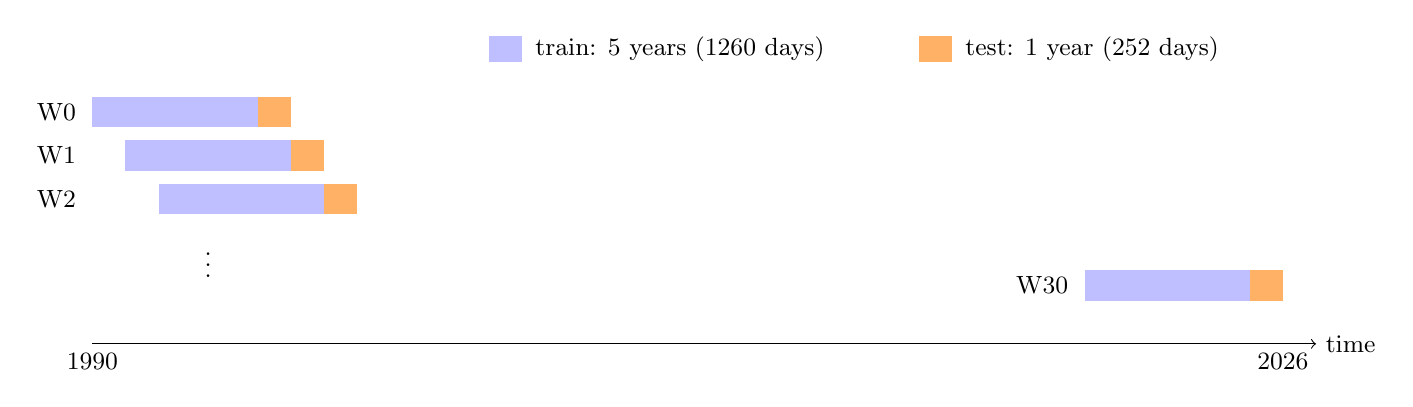
\begin{tikzpicture}[x=0.42cm,y=0.55cm]
  \foreach \i/\lab in {0/W0,1/W1,2/W2} {
    \fill[blue!25] (\i*1.0,-\i) rectangle ++(5,0.7);
    \fill[orange!60] (\i*1.0+5,-\i) rectangle ++(1,0.7);
    \node[left] at (-0.2,-\i+0.35) {\small \lab};
  }
  \node at (3.5,-3.0) {\small $\vdots$};
  \fill[blue!25] (30,-4) rectangle ++(5,0.7);
  \fill[orange!60] (35,-4) rectangle ++(1,0.7);
  \node[left] at (29.8,-3.65) {\small W30};
  \draw[->] (0,-5) -- (37,-5) node[right] {\small time};
  \node[below] at (0,-5) {\small 1990};
  \node[below] at (36,-5) {\small 2026};
  \fill[blue!25] (12,1.5) rectangle ++(1,0.6); \node[right] at (13.1,1.8) {\small train: 5 years (1260 days)};
  \fill[orange!60] (25,1.5) rectangle ++(1,0.6); \node[right] at (26.1,1.8) {\small test: 1 year (252 days)};
\end{tikzpicture}
\end{center}

\begin{itemize}
  \item Each window = train on 5 years, then test on the 1 year straight after it.
  \item Then slide everything forward by 1 year and do it again.
  \item \textbf{Test years never overlap.} Each test year is used once.
  \item \textbf{Training slices do overlap.} Window 1's training years are mostly the same as
        window 0's. (An older note said ``non-overlapping''; that is only true of the test
        slices.)
  \item \textbf{Every window trains a brand new model from random weights.} Nothing carries
        over from window to window.
  \item There are 31 windows. So the x-axis ``walk-forward window index'' runs 0 to 30, and
        it is really a \textbf{calendar of test years}.
\end{itemize}

Use this table to translate window numbers into history while you talk:

\begin{center}\small
\begin{tabular}{rlr@{\qquad}rlr}
\toprule
W & test year & B\&H Sharpe & W & test year & B\&H Sharpe \\
\midrule
0 & 1995 & +3.63 & 16 & 2011 & +0.02 \\
1 & 1996 & +1.67 & 17 & 2012 & +1.13 \\
2 & 1997 & +1.35 & 18 & 2013 & +2.08 \\
3 & 1998 & +1.14 & 19 & 2014 & +1.03 \\
4 & 1999 & +0.97 & 20 & 2015 & $-$0.14 \\
5 & 2000 (dot-com crash starts) & $-$0.58 & 21 & 2016 & +0.88 \\
6 & 2001 & $-$0.41 & 22 & 2017 & +2.74 \\
7 & 2002 & $-$1.07 & 23 & 2018 & $-$0.39 \\
8 & 2003 & +1.39 & 24 & 2019 & +2.10 \\
9 & 2004 & +0.81 & 25 & 2020 (COVID) & +0.40 \\
10 & 2005 & +0.35 & 26 & 2021 & +1.93 \\
11 & 2006 & +1.24 & 27 & 2022 (rate hikes) & $-$0.95 \\
12 & 2007 & +0.19 & 28 & 2023 & +1.71 \\
13 & 2008 (financial crisis) & $-$1.22 & 29 & 2024 & +1.71 \\
14 & 2009 & +0.86 & 30 & 2025 & +0.89 \\
15 & 2010 & +0.61 & & & \\
\bottomrule
\end{tabular}
\end{center}

\begin{sayit}
``Each point on the x-axis is one test year. Window 0 is 1995, window 13 is 2008, window 25
is 2020, window 30 is 2025. A fresh model is trained on the five years before each one and
then tested on that year without ever having seen it.''
\end{sayit}

\begin{qa}{``Why 5 years train and 1 year test?''}
``A 5 to 1 ratio is inside the usual walk-forward range for daily financial data, it gives
the agent enough history to learn from, and one-year tests give me 31 separate
out-of-sample years, which is a decent number of independent checks.''
\end{qa}

% ============================================================================
\section{The 868 models, the seeds, and what ``2604'' means}

This is the section for the question that threw you last time.

\subsection{Where 868 comes from}

For each learner there are three things that vary. Multiply them:
\[
\underbrace{4}_{\text{configurations}} \times \underbrace{7}_{\text{seeds}} \times
\underbrace{31}_{\text{windows}} = 868 \text{ trained models.}
\]

\begin{center}
\begin{tabular}{llll}
\toprule
Sweep & the 4 configurations & 7 seeds & 31 windows \\
\midrule
LSTM (RQ1) & h64L1, h64L2, h128L1, h128L2 & 0 to 6 & 1995 to 2025 \\
PPO + FS & $k$ = 3, 5, 10, 20 & 0 to 6 & 1995 to 2025 \\
PPO + AS & $k$ = 3, 5, 10, 20 & 0 to 6 & 1995 to 2025 \\
\bottomrule
\end{tabular}
\end{center}

Three sweeps $\times$ 868 = \textbf{2604 models}, every one trained from scratch.

\begin{sayit}
``The 868 are not 868 training iterations of one model. They are 868 separate models. For
each of the 4 settings, I train 7 copies with different random seeds, and I do that
separately in each of the 31 test years. 4 times 7 times 31 is 868.''
\end{sayit}

\subsection{What a seed is}

A seed is the starting number for the random number generator. Changing it changes every
random choice in training, while keeping the data and settings identical:
\begin{itemize}
  \item the network's random starting weights,
  \item the order of the minibatches,
  \item for PPO, the random actions sampled while exploring during training,
  \item for the LSTM with 2 layers, which connections dropout switches off.
\end{itemize}

Why 7: with 1 seed you cannot tell skill from luck. RL papers usually report 5 to 10 seeds.
Started with 3 for prototyping, then went to 7 for the reported results.

Why it helps the comparison: \textbf{all three sweeps use the same seed list (0 to 6) and the
same 31 windows.} So for FS and AS at the same $k$, I can line up ``same year, same seed''
pairs and compare them directly. Section 9 does exactly that.

\begin{qa}{``So what is one training run of PPO, in numbers?''}
``One model trains for 100,000 timesteps on its 1260-day training slice. That is about 79
passes through those five years. PPO collects 2048 steps, then does 10 epochs of minibatch
updates with batch size 64 and learning rate 0.0003, and repeats. That is about 49 updates
per model. Everything else is the Stable-Baselines3 default: $\gamma=0.99$, GAE $\lambda=0.95$,
clip range 0.2, no entropy bonus, a 64 by 64 MLP. FS and AS use exactly the same PPO
settings; only the memory wrapper differs.''
\end{qa}

\begin{qa}{``How was the PPO configuration chosen? Did you tune it?''}
``No, it is the library default with the learning rate and batch size written out, and it is
held fixed across both sweeps on purpose. The only thing I swept for RL is the memory budget
$k$, because $k$ is the variable the research question is about. Tuning PPO separately for FS
and AS would make it unclear whether a difference came from memory or from tuning.''
\end{qa}

\begin{honest}
The LSTM got a small hyperparameter search (4 shapes) and the PPO agents did not. That is
defensible (it makes the baseline strong, not weak), but say it plainly.
\end{honest}

\subsection{Cost}
Average training time per model on CPU: LSTM about 4 seconds, PPO + FS about 156 seconds,
PPO + AS about 484 seconds. \textbf{AS is about three times slower to train than FS}, because
its action space and its policy head are larger. That is a real cost to report.

% ============================================================================
\section{Sharpe ratio, explained to an RL person}

\subsection{The formula}
For one test year, take the 252 daily rewards $r_1, \ldots, r_{252}$. Then
\[
\text{Sharpe} = \sqrt{252}\; \frac{\text{mean}(r)}{\text{std}(r)}.
\]
The risk-free rate is set to 0, which is normal in research comparisons. The $\sqrt{252}$
only converts a daily number into a yearly one. It is the same for every model, so it does
not change who wins.

\subsection{The one sentence that lands with an RL person}

\begin{sayit}
``Sharpe is the signal-to-noise ratio of the reward stream. The numerator is the average
reward per step, which is what RL normally cares about. The denominator is how much that
reward wobbles. So Sharpe asks: how much reward did you get per unit of noise you had to
sit through?''
\end{sayit}

Then give the two-agent example:
\begin{sayit}
``Two agents both make 5\% in a year. One gets there smoothly, the other swings up and down by
15\%. Total reward is the same. Sharpe says the smooth one is better, because you could
safely put more money behind it.''
\end{sayit}

\subsection{Is it a valid metric to go by? Yes, with three caveats}

\textbf{Why it is valid here:}
\begin{itemize}
  \item \textbf{It does not care about position size.} If an agent doubled every position,
        its mean and its standard deviation both double, so its Sharpe is unchanged. That
        makes it a fair way to compare agents that bet with different conviction.
  \item \textbf{It is the standard in finance}, so the numbers can be compared to buy and hold
        and to published work.
  \item \textbf{I do not rely on it alone.} I also report cumulative return (raw total reward),
        max drawdown (worst loss) and flips (trading behaviour).
\end{itemize}

\textbf{Caveat 1: the agent was not trained to maximise Sharpe.} PPO maximises discounted
total reward, which is the numerator only. So there is a mismatch between what the agent
optimises and how I score it. Related work (Moody and Saffell) trains directly on a
``differential Sharpe'' reward; that is an obvious extension.

\textbf{Caveat 2: one year of Sharpe is a noisy measurement.} A Sharpe ratio estimated from
one year of daily data has a standard error of roughly 1 (Lo, 2002: about
$\sqrt{(1 + \text{SR}^2/2)/\text{years}}$, which is about 1 for one year). This is the main
reason the error bars on every bar chart are about $\pm 1.2$. It is not that the models are
broken; it is that a single year cannot pin a Sharpe down more precisely than that.

\textbf{Caveat 3: it treats good and bad swings the same.} A big up day counts as ``risk''
just like a big down day. Sortino ratio fixes this; max drawdown covers the downside part.

\begin{qa}{``Why not just report the RL return?''}
``I do: cumulative return is exactly the undiscounted sum of rewards in the test year. But
on its own it hides risk. An agent can earn a lot by being long all the time in a bull
market, which is just buy and hold. Sharpe tells me whether the return came with less
noise.''
\end{qa}

\subsection{What a Sharpe number feels like}
Below 0: losing money after accounting for risk. Around 0.5: modest. Around 1: good.
Above 2: excellent, and rare over many years. Buy and hold over these 31 years averages
0.84 per year.

% ============================================================================
\section{Plot by plot}

Every plot below follows the same pattern. Read the blue box first, then practise the green
box aloud.

% ---------------------------------------------------------------------------
\subsection{The ``whisker'' bar chart: LSTM champion picker}
\fig{rq1_lstm_sweep/seed_7/aggregate_sharpe_by_hp.png}{0.85}
\begin{axes}
\textbf{x-axis:} the four LSTM shapes. Each tick label has three lines: the ID (hp0), the
shape (h64L1 = hidden 64, one layer), and the nominal dropout (d0.2).\\
\textbf{y-axis:} Sharpe ratio.\\
\textbf{Each bar:} the \emph{mean} of 217 Sharpe values for that shape (7 seeds $\times$ 31
test years).\\
\textbf{Each whisker (the vertical line with caps):} one standard deviation of those 217 values,
above and below the mean. It is \emph{not} a confidence interval and \emph{not} a min-max.\\
\textbf{Red dashed line:} buy and hold, averaged over the 31 years (0.841).\\
\textbf{Green outline:} the champion, h128L1, mean Sharpe +0.208.
\end{axes}
\begin{sayit}
``The x-axis is the four LSTM shapes I tried: hidden size 64 or 128, and one or two layers.
Each bar is the average Sharpe over 7 seeds and 31 test years, so 217 numbers, and the
whisker is one standard deviation of those 217. The best is hidden 128 with one layer at
0.21. All four sit well below buy and hold, and the whiskers are huge, which tells you the
LSTM has very little real forecasting signal here. I tuned it anyway so that RQ1 is
against a fair baseline, not a weak one.''
\end{sayit}
\begin{qa}{``Why are the whiskers so big?''}
``Two reasons. First, they mix 31 very different market years. 2008 and 2017 do not look
alike. Second, one year of Sharpe is itself noisy, with a standard error of about 1. For the
LSTM, the seed-to-seed spread inside the same year is also large, about 1.0, so the LSTM is
genuinely unstable from seed to seed. Figure \ref{fig:spread} breaks this down.''
\end{qa}

% ---------------------------------------------------------------------------
\subsection{Per-shape timelines (hp\_0 to hp\_3, Sharpe and cumulative return)}
These live in \texttt{results/rq1\_lstm\_sweep/seed\_7/}. There is one per LSTM shape.
\begin{axes}
\textbf{x-axis:} walk-forward window index, so test year (0 = 1995, 30 = 2025).\\
\textbf{y-axis:} Sharpe (or cumulative return in the \texttt{cumret} version) for that year.\\
\textbf{Solid line:} the median over the 7 seeds in that year.\\
\textbf{Shaded band:} the lowest to the highest seed in that year (min to max).\\
\textbf{Dashed line:} buy and hold in that year.
\end{axes}
\begin{sayit}
``This shows one LSTM shape year by year. The line is the middle seed, the shaded band is
the range from worst to best seed. Where the band is wide, the result in that year depends
heavily on luck of initialisation.''
\end{sayit}

% ---------------------------------------------------------------------------
\subsection{FS champion picker across $k$}
\fig{rq1/02_fs_champion_bar.png}{0.62}
\begin{axes}
Same layout as the LSTM chart. \textbf{x-axis:} memory budget $k$ for Frame Stacking, sorted
best first. \textbf{Bars:} mean Sharpe over 217 runs. \textbf{Whiskers:} $\pm$1 std.
\textbf{Green:} champion, $k=3$, Sharpe +0.484.
\end{axes}
\begin{sayit}
``For Frame Stacking, the shortest memory, three days, did best, at 0.48. Giving it more
history made it slightly worse: 0.44 at five, about 0.31 to 0.32 at ten and twenty. A longer
fixed window mostly adds noise.''
\end{sayit}

% ---------------------------------------------------------------------------
\subsection{RQ1 head to head}
\fig{rq1/03_rq1_head_to_head.png}{0.62}
\begin{axes}
\textbf{x-axis:} three contenders: LSTM champion, FS champion, buy and hold.
\textbf{y-axis:} Sharpe, mean $\pm$ std over 217 runs. B\&H has no whisker here because it
has no seeds; it is the same every run.
\end{axes}
\begin{sayit}
``This is RQ1 in one picture. PPO with Frame Stacking averages 0.48, the LSTM averages 0.21.
So the RL framing does better, by about 0.28. Neither beats buy and hold.''
\end{sayit}
\begin{honest}
Paired by test year, FS beats the LSTM in 20 of 31 years, but the difference is not
statistically significant (paired $t$-test $p \approx 0.10$, Wilcoxon $p \approx 0.14$).
Say ``RL is ahead'', not ``RL is proven better''.
\end{honest}

% ---------------------------------------------------------------------------
\subsection{RQ1 Sharpe timeline}
\fig{rq1/04_sharpe_timeline_lstm_vs_fs.png}{0.9}
\begin{axes}
\textbf{x-axis:} test year (window index). \textbf{y-axis:} Sharpe in that year.
\textbf{Orange:} LSTM champion. \textbf{Green:} FS champion. Lines are seed medians, bands are
min to max over seeds. \textbf{Red dashed:} buy and hold.
\end{axes}
\begin{sayit}
``Two things to notice. First, the green FS line often sits exactly on the buy-and-hold line,
especially in windows 0 to 4 and in the bull years at the end. In those years the agent
learned to just stay long. Second, the orange LSTM band is much wider: its seeds disagree a
lot, and it has some bad years where FS does not, like windows 25 and 26.''
\end{sayit}
\begin{qa}{``So is your RL agent just buy and hold?''}
``Partly, in bull years, yes, and I think that is the honest reading. FS at $k=3$ is long
about 76\% of days. Where it differs from buy and hold is in a few hard years, like 2008
(window 13) and 2011 (window 16), where it does clearly better than buy and hold. That is where any memory benefit has to show up.''
\end{qa}

% ---------------------------------------------------------------------------
\subsection{RQ1 equity curves}
\fig{rq1/05_equity_curves.png}{0.85}
\begin{axes}
\textbf{x-axis:} test year (window index). \textbf{y-axis:} money, where 1.0 is what you started
with. Each line chains the 31 test years together: the average log return of each year is
added up and turned back into a growth factor.
\end{axes}
\begin{sayit}
``This is the `how much would one rand have grown to' picture, if you had run each champion
year after year. Buy and hold ends far above everything, because these 31 years were mostly
a rising market and being long every day is very hard to beat in that setting.''
\end{sayit}
\begin{honest}
The agents' curves use the \emph{average} over seeds each year. A real trader would run one
seed, not the average, so this is a smoothed picture.
\end{honest}

% ---------------------------------------------------------------------------
\subsection{RQ1 position distribution}
\fig{rq1/06_position_distribution.png}{0.6}
\begin{axes}
\textbf{x-axis:} the three positions. \textbf{y-axis:} fraction of all test days spent in each.
Orange is the LSTM, green is FS.
\end{axes}
\begin{sayit}
``The LSTM is never flat, because it turns a forecast into a position by its sign, and a
forecast is almost never exactly zero. It goes about 57\% long and 43\% short, so it is close
to a coin flip with a long tilt. The FS agent is long about 76\% of the time, flat 7\%, short
17\%. It learned the market usually rises.''
\end{sayit}

% ---------------------------------------------------------------------------
\subsection{RQ2: AS versus FS at each $k$ (the main bar chart)}
\fig{rq2/01_as_vs_fs_by_k_bars.png}{0.9}
\begin{axes}
\textbf{x-axis:} memory budget $k$. At each $k$ there are two bars side by side: blue is FS,
purple is AS, with the same $k$. \textbf{y-axis:} mean Sharpe over 217 runs.
\textbf{Whiskers:} $\pm$1 std. \textbf{Red dashed:} buy and hold.
\end{axes}
\begin{center}\small
\begin{tabular}{rcccc}
\toprule
$k$ & FS mean Sharpe & AS mean Sharpe & AS minus FS & AS better in (of 31 years) \\
\midrule
3 & 0.484 & 0.459 & $-$0.02 & 13 \\
5 & 0.435 & \textbf{0.515} & +0.08 & 16 \\
10 & 0.310 & 0.447 & +0.14 & 19 \\
20 & 0.321 & 0.437 & +0.12 & 16 \\
\bottomrule
\end{tabular}
\end{center}
\begin{sayit}
``Each pair of bars has the same memory size, so this is the matched-budget comparison. At
three slots FS is very slightly ahead. At five, ten and twenty, AS is ahead. The more
interesting pattern is that FS gets worse as you give it more memory, from 0.48 down to
about 0.31, while AS stays roughly flat around 0.44 to 0.52. So learned memory seems to
cope with a bigger budget better than a fixed window does.''
\end{sayit}

% ---------------------------------------------------------------------------
\subsection{The paired view (new figure, made for this guide)}
\fig{paired_difference.png}{0.85}
\begin{axes}
\textbf{x-axis:} memory budget $k$. \textbf{y-axis:} AS Sharpe minus FS Sharpe in the
\emph{same} test year (each averaged over its 7 seeds). \textbf{Grey dots:} the 31 test years.
\textbf{Black dot:} the average difference. \textbf{Black whisker:} a 95\% bootstrap interval
for that average. \textbf{Red line:} zero, meaning no difference.
\end{axes}
\begin{sayit}
``This is the fairer way to compare, because it removes the effect of the year. If a year was
bad for everybody, it is bad for both, and the difference cancels it. The averages are above
zero at five, ten and twenty, but every interval still crosses zero. So the direction is
consistent, but I cannot claim it is significant yet.''
\end{sayit}
\begin{qa}{``Is AS significantly better than FS?''}
``No, not at any single $k$. The paired $t$-test $p$-values are between 0.23 and 0.71. I would
call it directional evidence. To make it firm I would need either more test years or a
less noisy metric, because a one-year Sharpe has a standard error near 1 on its own.''
\end{qa}

% ---------------------------------------------------------------------------
\subsection{Where the error bars come from (new figure)}
\fig{where_spread_comes_from.png}{0.9}
\label{fig:spread}
\begin{axes}
\textbf{x-axis:} each configuration. \textbf{y-axis:} standard deviation of Sharpe.
\textbf{Orange bar:} how much the 7-seed average moves from one test year to the next (the
market). \textbf{Grey bar:} how much the 7 seeds disagree within the same year (luck of
initialisation).
\end{axes}
\begin{sayit}
``For the RL agents, most of the error bar is the market, not the seed. In the same year,
different seeds mostly agree. For the LSTM it is the other way around: its seeds disagree more
than its years do, so the LSTM is the unstable learner here. This is also why I compare AS
and FS year by year: it removes the orange part.''
\end{sayit}

% ---------------------------------------------------------------------------
\subsection{Sharpe against $k$, as lines}
\fig{rq2/02_sharpe_vs_k_lines.png}{0.7}
\begin{axes}
\textbf{x-axis:} memory budget $k$, on a log scale (so 3, 5, 10, 20 are evenly spread).
\textbf{y-axis:} mean Sharpe. \textbf{Shaded bands:} $\pm$1 std. Blue FS, purple AS, red dashed
buy and hold.
\end{axes}
\begin{sayit}
``Same numbers as the bar chart, drawn as a trend. The blue FS line falls as memory grows. The
purple AS line stays flatter. The shaded bands overlap almost completely, which is the same
`directional, not significant' message.''
\end{sayit}

% ---------------------------------------------------------------------------
\subsection{Retention: which slot does AS throw away? (corrected figure)}
\fig{retention_corrected.png}{1.0}
\begin{honest}
\textbf{The version of this plot in \texttt{plots/rq2/03\_retention\_histogram\_by\_k.png} is
wrong.} The plotting code sorts column names as text, so it reads \texttt{mem\_slot\_0},
\texttt{mem\_slot\_1}, \texttt{mem\_slot\_10} \ldots\ instead of 0, 1, 2. For $k=3, 5, 10$ that
means it shows two real bars and then empty columns as zeros, and for $k=20$ the bars are in
the wrong order. The figure above reads the same CSV in the right order. The fix in
\texttt{generate\_plots.py} is one line: build the column list as
\texttt{[f"mem\_slot\_\{i\}" for i in range(k)]} instead of sorting strings. Tell Geraud you
found and fixed this. Do not show the old one.
\end{honest}
\begin{axes}
\textbf{What a ``slot'' is here.} AS keeps $k$ observations in a list ordered by age. Slot 0 is
the oldest one still kept; slot $k-1$ is the newest. Each day the agent removes one slot, the
others shift up, and today's observation goes in at the end.\\
\textbf{x-axis:} slot position, oldest (0) to newest ($k-1$).\\
\textbf{y-axis:} fraction of all overwrite decisions, over every test day of every seed and
window.\\
\textbf{Red dashed line:} $1/k$, what you would see if the agent picked a slot at random.
\end{axes}
\textbf{Three reference patterns to keep in your head:}
\begin{itemize}
  \item \textbf{All the mass on slot 0} = always throw away the oldest = \textbf{exactly Frame
        Stacking}.
  \item \textbf{Flat at $1/k$} = random eviction, no preference.
  \item \textbf{Mass towards the right} = keeps throwing away the newest and \emph{holds on to
        older observations}.
\end{itemize}
What the data shows: the third pattern, and it gets stronger as $k$ grows. At $k=10$ the
newest slot is thrown away 18\% of the time and the oldest only 4\%. At $k=5$ it is 28\% versus
10\%.
\begin{sayit}
``If AS had learned nothing, this would be flat. If it had learned to copy Frame Stacking,
everything would be on the left, on slot 0. Instead the agent most often throws away the
\emph{newest} observation and rarely the oldest. In other words it holds on to older
observations for longer than a sliding window would. So it is not behaving like Frame
Stacking, and it is not random.''
\end{sayit}
\begin{honest}
Two cautions. First, at test time the memory starts filled with copies of the first
observation of the year, so if an agent almost always evicts the newest slot, the ``old''
slots it keeps may just be those starting copies, and the agent is effectively looking at
today only. Check this in \texttt{steps.csv} before claiming the agent keeps
\emph{meaningful} old events. Second, at $k=3$ about 69\% of runs put more than 90\% of their
choices on one slot: the evaluation is deterministic (\texttt{deterministic=True}), so many
runs commit to one fixed rule.
\end{honest}

% ---------------------------------------------------------------------------
\subsection{Champion Sharpe timeline: AS $k=5$ against FS $k=3$}
\fig{rq2/04_sharpe_timeline_as_vs_fs.png}{0.9}
\begin{axes}
Same layout as the RQ1 timeline. \textbf{x-axis:} test year. \textbf{y-axis:} Sharpe that year.
Purple AS $k=5$, blue FS $k=3$, median over seeds, bands min to max. Red dashed buy and hold.
\end{axes}
\begin{sayit}
``In windows 0 to 4 both agents sit on buy and hold, they just stay long. The differences
appear in the middle years, roughly 2003 to 2014, where AS is above FS more often, for
example windows 14, 16, 18 and 19. AS also has one very wide band in window 24, 2019, where one
seed did badly; that is a single-seed failure, not the median.''
\end{sayit}

% ---------------------------------------------------------------------------
\subsection{Champion equity curves}
\fig{rq2/05_equity_curves_champions.png}{0.85}
\begin{sayit}
``Same `growth of one rand' picture. AS $k=5$ ends at about 4.5 times, FS $k=3$ at about 4.2
times, buy and hold at about 15 times. The two agents track each other closely until around
2003, and the AS line pulls slightly ahead after that and stays ahead.''
\end{sayit}

% ---------------------------------------------------------------------------
\subsection{Position flips}
\fig{rq2/06_position_flips_by_k.png}{0.65}
\begin{axes}
\textbf{x-axis:} memory budget $k$. \textbf{y-axis:} average number of position changes in one
252-day test year. Blue FS, purple AS.
\end{axes}
\begin{center}\small
\begin{tabular}{rcc}
\toprule
$k$ & FS flips per year & AS flips per year \\
\midrule
3 & 32.6 & 28.6 \\
5 & 54.4 & 31.2 \\
10 & 87.5 & 40.2 \\
20 & 117.5 & 52.3 \\
\bottomrule
\end{tabular}
\end{center}
\begin{sayit}
``This is the clearest difference between the two mechanisms. With more memory, the Frame
Stacking agent changes its mind a lot more: 117 times a year at $k=20$. The AS agent at the
same budget changes about 52 times, less than half. So learned memory gives a much steadier
trader, and that matters, because every flip costs money.''
\end{sayit}

% ---------------------------------------------------------------------------
\subsection{Training diagnostics}

\textbf{Entropy.}
\fig{training_diagnostics/01_entropy_decay.png}{0.8}
\begin{axes}
\textbf{x-axis:} training timesteps for one model (0 to 100,000). \textbf{y-axis:} SB3's
\texttt{entropy\_loss}. Each faint line is one model.
\end{axes}
\begin{honest}
The plot title says ``lower means more decisive''. That is backwards. SB3's
\texttt{entropy\_loss} is \emph{minus} the entropy. So a line rising towards 0 means the
policy is becoming \emph{more} decisive. Fix the title.
\end{honest}
\begin{sayit}
``Every curve starts at the value of a completely random policy. For FS that is minus log 3,
about minus 1.1, because it has three actions. For AS it starts lower because it also picks a
slot: minus log 3 minus log $k$. That is why there are four purple bands, one per $k$. All of them
rise during training, so every policy becomes more decisive. The FS ones get close to zero,
almost deterministic. The AS ones stay far from zero, so the memory choice is still quite
spread out at the end of training, especially for large $k$.''
\end{sayit}

\textbf{Value loss and explained variance.}
\fig{training_diagnostics/03_explained_variance.png}{0.8}
\begin{sayit}
``Explained variance measures how well the critic predicts the returns it will get. It starts
very negative, which just means the untrained critic is worse than guessing the average, and
within the first few updates it climbs to around zero and stays a little above zero. So the
critic learns very little. That is what I would expect, because tomorrow's market return is
close to unpredictable from today's VIX.''
\end{sayit}
\begin{honest}
The project notes quote a rule of thumb that explained variance above 0.5 is healthy. Your
runs do not reach that. Do not hide it: explain it with the low predictability of the data
(see the correlation plot next). Value loss (\texttt{02\_value\_loss.png}) tells the same
story: it drops early and then flattens.
\end{honest}

% ---------------------------------------------------------------------------
\subsection{Data-integrity plots (quick)}

These are in \texttt{plots/data\_integrity/}. Know one sentence for each.
\begin{itemize}
  \item \textbf{01 price series.} VIX on top (spikes in 2008, 2020), S\&P below (long rise).
        ``The regimes are visible by eye.''
  \item \textbf{02 and 03 histograms and KDE.} x-axis: daily log return. y-axis: count or
        density. ``VIX changes are wider and skewed to the right, because it spikes up
        suddenly. S\&P returns are narrow and fat-tailed.''
  \item \textbf{04 boxplots by decade.} x-axis: decade. y-axis: log return. ``The middle of
        the distribution is stable, the spread changes by decade.''
  \item \textbf{05 autocorrelation.} x-axis: lag in days. y-axis: correlation of a series
        with itself shifted by that many days. ``Almost zero at every lag. Returns do not
        predict themselves, as expected.''
  \item \textbf{06 rolling mean and std.} ``The mean stays near zero, the volatility jumps in
        2008 and 2020. So the data is stable in mean but not in variance, which is why I
        retrain per window.''
\end{itemize}

\textbf{07 rolling correlation, the important one.}
\fig{data_integrity/07_rolling_correlation_vix_sp.png}{0.85}
\begin{axes}
\textbf{x-axis:} date. \textbf{y-axis:} correlation over the past 252 days between
\emph{today's} VIX log return and \emph{tomorrow's} S\&P log return.
\end{axes}
\begin{honest}
\texttt{DATA\_TERMINAL.md} and the speaker notes say this correlation is about $-0.7$ to
$-0.8$. \textbf{That is not what this plot shows.} $-0.7$ is the \emph{same-day} relationship
(VIX up, S\&P down, on the same day). This plot shows the \emph{predictive} relationship,
today's VIX against tomorrow's S\&P, and it stays between about $-0.2$ and $+0.25$, mostly
near zero, and even changes sign. Correct the note, and do not say ``VIX is strongly
informative about the next day''.
\end{honest}
\begin{sayit}
``On the same day VIX and the S\&P move strongly against each other. But what the agent can
trade on is tomorrow, and today's VIX change is only weakly related to tomorrow's S\&P
return, and the sign of that relationship flips over time. So this is a hard, low-signal,
changing environment. That is exactly the kind of setting where we did not know if Adaptive
Stacking would still help, and it also explains why every learner sits close to buy and
hold.''
\end{sayit}

% ============================================================================
\section{What the numbers really support}

\subsection{Headline table}
\begin{center}\small
\begin{tabular}{lcccc}
\toprule
 & Mean Sharpe & Std & Mean max drawdown & Flips per year \\
\midrule
Buy and hold & 0.841 & n/a & 0.150 & 0 \\
LSTM champion (h128L1) & 0.208 & 1.249 & & 40.4 \\
FS champion ($k=3$) & 0.484 & 1.194 & 0.151 & 32.6 \\
AS champion ($k=5$) & \textbf{0.515} & 1.188 & 0.152 & 31.2 \\
\bottomrule
\end{tabular}
\end{center}

\subsection{Claims you can make, and how strongly}

\begin{center}\small
\begin{tabular}{p{7.2cm}p{2.4cm}p{4.8cm}}
\toprule
Claim & Strength & Evidence \\
\midrule
RL (FS) does better than the tuned LSTM. & Directional & +0.28 Sharpe, 20/31 years,
  $p\approx0.10$ \\
AS does better than FS at $k=5,10,20$. & Directional & +0.08 to +0.14, intervals cross 0 \\
FS gets worse as $k$ grows; AS does not. & Directional & 0.48 to 0.31 vs 0.52 to 0.44 \\
AS trades much less than FS at large $k$. & \textbf{Strong} & 52 vs 117 flips at $k=20$ \\
AS does not behave like FIFO; it keeps older slots. & \textbf{Clear}, with caveat & corrected
  retention plot \\
Nothing beats buy and hold. & Clear & 0.84 vs 0.52 at best \\
Max drawdown: no difference. & Clear & 0.151 vs 0.152 vs 0.150 \\
\bottomrule
\end{tabular}
\end{center}

\begin{sayit}
``My honest conclusion so far: learned memory does not hurt, it is ahead at three of four
budgets, and it clearly changes \emph{how} the agent trades: steadier positions and longer
retention. But in a market this noisy, 31 test years are not enough to call the Sharpe gain
significant. I'd present it as directional evidence plus a clear behavioural difference.''
\end{sayit}

\begin{qa}{``Is a negative or null result acceptable for the project?''}
You asked this yourself back in May. Your own position then was: yes, a result showing where
Adaptive Stacking's assumptions stop paying off is still a contribution. Say: ``It works on
stationary benchmarks; here the gain shrinks to something I cannot separate from noise,
although behaviour clearly changes. That tells us something about where the method's
advantage comes from.''
\end{qa}

% ============================================================================
\section{Things to raise yourself}

Bring these up before he does. Each one, said calmly, makes you look in control.

\begin{enumerate}
  \item \textbf{The retention plot bug.} Found it, fixed it, here is the corrected figure.
  \item \textbf{The summary.json champion bug.} The champion in \texttt{summary.json} only reflects
        the last resumed session, because \texttt{train.py} builds it from the runs it trained
        in that session. \texttt{windows.csv} has all 868 rows and every number in this guide
        comes from it.
  \item \textbf{No sealed final holdout.} Walk-forward was used, but the last two years were not
        locked away untouched. Ask him if documenting it is enough or if he wants a re-run.
  \item \textbf{Not statistically significant.} Paired tests, $p$ between 0.23 and 0.71 for
        RQ2, about 0.10 for RQ1.
  \item \textbf{Inputs not standardised for PPO.} The LSTM z-scores its inputs with
        training-slice statistics. The PPO agents receive raw VIX log returns. Both FS and AS
        get the same raw inputs, so RQ2 is still fair, but RQ1 has this small asymmetry.
  \item \textbf{The agent cannot see its own position}, yet its cost depends on it.
  \item \textbf{Old wording to correct}: ``24 years'' should be 36 years of data and 31 test
        years; ``non-overlapping windows'' applies to test years only; the $-0.7$ correlation is
        same-day, not predictive; the entropy plot title is reversed; ``d0.2'' had no effect on
        1-layer LSTMs.
  \item \textbf{Cost.} AS takes about 3 times longer to train than FS.
\end{enumerate}

% ============================================================================
\section{Question drill}

Cover the answers, read the question, answer aloud, then check.

\begin{qa}{What is the x-axis on the bar charts?}
The configurations: four LSTM shapes, or the four values of $k$. Each bar is a mean over 217
runs (7 seeds $\times$ 31 test years), each whisker is one standard deviation.
\end{qa}
\begin{qa}{What is the x-axis on the timelines and equity curves?}
The walk-forward window, which is the test year: 0 is 1995, 30 is 2025.
\end{qa}
\begin{qa}{What are the 800-something runs?}
868 separate models per learner: 4 settings $\times$ 7 seeds $\times$ 31 windows. Three
learners, so 2604.
\end{qa}
\begin{qa}{What does a seed change?}
Starting weights, minibatch order, exploration noise during PPO training, dropout masks. Not
the data, not the settings.
\end{qa}
\begin{qa}{Why does Sharpe make sense for an RL agent?}
It is the signal-to-noise ratio of the reward stream. It rewards earning the same total reward
with less variation, and it does not change if you scale position size.
\end{qa}
\begin{qa}{Why didn't you give AS a ``skip'' option (keep everything)?}
Because skipping would always be the safe choice and the memory head would learn nothing. Forcing
an overwrite every step makes different memory choices lead to different outcomes, which is
what produces a learning signal.
\end{qa}
\begin{qa}{Why is the FS champion at the smallest $k$?}
Tomorrow's return is barely related to today's VIX, so extra fixed history is mostly noise to
the network, and it starts flipping position more. That is also where a selective memory
should help most, and the flip numbers support that.
\end{qa}
\begin{qa}{Why can't anything beat buy and hold?}
The test period is mostly a rising market, and the predictive signal from VIX is weak. The
project asks which memory is better, not whether I built a profitable fund.
\end{qa}
\begin{qa}{How do you know you didn't leak future data?}
The reward uses tomorrow's return through an explicit one-day shift; every window trains a
fresh model only on data before its test year; LSTM standardisation uses training-slice
statistics only.
\end{qa}
\begin{qa}{What would you do with more time?}
A significance test across more years or more assets; a sealed holdout; check in
\texttt{steps.csv} what the AS agent actually keeps; a Sharpe-based reward; and giving the agent
its own position as an input.
\end{qa}

% ============================================================================
\section{A 10-minute talk you can give tomorrow}

\begin{enumerate}
  \item \textbf{(1 min) The question.} The 30-second version from Section 1.
  \item \textbf{(1 min) The data and the MDP.} Two streams, one-day shift, 9188 days.
        Show the rolling correlation plot: hard, weak, changing signal.
  \item \textbf{(1 min) The design.} Walk-forward diagram. 4 $\times$ 7 $\times$ 31 = 868 per
        learner. Same seeds and windows everywhere, PPO settings fixed.
  \item \textbf{(2 min) RQ1.} LSTM picker (explain the axes first), then head to head.
        ``RL is ahead, not significantly.''
  \item \textbf{(3 min) RQ2.} AS vs FS bars, then the paired plot, then flips, then the corrected
        retention plot. ``Directional on Sharpe, clear on behaviour.''
  \item \textbf{(1 min) Honesty slide.} The list from Section 10.
  \item \textbf{(1 min) Next.} Report in Overleaf (IEEE template), poster, and the one question for
        him: holdout re-run, or document it?
\end{enumerate}

\begin{sayit}
If you lose your place: ``LSTM is the control, Frame Stacking is the standard, Adaptive
Stacking is the contribution.'' Then go to the next plot and start with its axes.
\end{sayit}

\vspace{1em}
\hrule
\small
\textit{Sources for every number in this guide:} \texttt{results/rq1\_lstm\_sweep/windows.csv},
\texttt{results/rq\_rl\_fs\_sweep/windows.csv}, \texttt{results/rq\_rl\_as\_sweep/windows.csv},
the sweep configs in \texttt{configs/}, and \texttt{src/}. New figures are made by
\texttt{defence/make\_defence\_figures.py}.

\end{document}
